\chapter{單一語音離散表徵與音位的關係}
{

{

  HuBERT \cite{hsu_hubert_2021, hsu_hubert_2021-2} 和 Wav2vec 2.0 \cite{baevski2020wav2vec} 等語音基石模型的成功,不僅在語音任務上達到了前所未有的表現,還促進了語音表徵離散化的發展。由此產生的「無文字(Textless)」架構 \cite{noauthor_textless_2021, lakhotia_generative_2021, lakhotia_generative_2021-1},讓人們在處理語音訊號時,有了連續表徵以外的新選擇。離散形式的表徵可以直接應用文字領域發展的技術,如機器翻譯、生成式模型等,為語音技術帶來新的突破。另一方面,基於離散「符記(Token)」的共同形式,離散語音表徵可以更好的整合文字資料,促成多模態領域的發展。跨模態離散表徵的成功,甚至驅使影像領域也開始發展離散表徵,如探討唇語的 AV-HuBERT \cite{shi2021learning} 等等,展現了離散表徵在資料處理上的優勢。

        此外,除了技術的角度切入,這樣的技術也可以探討離散語音表徵成功背後的可能因素,以及它們與語言學對人類語音理解之間的差異,甚至是進一步利用這些技術協助更細緻的探討人類的語音現象。因此,原先在連續語音表徵上的語音學分析,也開始關注離散表徵在多大程度上能描述語音現象,將其列入考量,成為除了連續語音特徵和時頻譜之外的另一個選擇。

\section{相關研究}  

\subsection{無文字與離散語音表徵}

  自 HuBERT 帶起的研究之後,出現了愈來愈多離散表徵相關的研究\cite{10097097, abdullah23_interspeech, chang_exploration_2023, liu2024dinosr, zhang2024speechtokenizer, huang2023repcodec} 。它們在提出自己的離散表徵時,也會採取 HuBERT 的衡量方式,來驗證這些離散單元與語音中的內容及人類對語音的詮釋之間,具有一定程度的相關性,並從資訊理論(Information Theory)的角度,證明這些離散單元確實具備區分不同語音資訊的能力。

\subsection{語音學分析}

  由於語音處理本身最終是針對人類語音,因此有一群研究者通過對人類語音的理解,將這些知識應用在分析模型如何對語音訊號建構表徵之上\cite{deseyssel22_interspeech, wells_phonetic_2022, 10097097, abdullah23_interspeech} 。基於這些作品對語音離散表徵的興趣和探討,本論文也先透過過往幾個常用來分析語音表徵的方式,特別是 HuBERT \cite{hsu_hubert_2021-2} 提出的標準進行初步的分析。


\section{衡量指標}

  本次研究主要探討純度(Purity)、熵(Entropy)和相互資訊(Mutual Information,MI)等指標,這些指標在 HuBERT 中被採用 \cite{hsu_hubert_2021, hsu_hubert_2021-2},用以比對機器學習過程中得到的虛擬標註與人類標註之間的相關性(Correlation),接下來將詳細解釋這些指標的定義。

        包含聲學特徵與語音基石模型,不論採用何種方式獲得語音表徵,語音訊號皆是以音框(Frame)為基本單位進行處理。具體而言,給予一段聲音訊號,語音處理系統會將這段訊號按照固定時間切割成多個片段分別處理,這些片段的長度被稱之為時間解析度(Time Resolution)。因此,對於任意一段語句(Utterance),系統會將訊號轉換成一連串的向量 $\boldsymbol{x} = [x_1, \cdots\cdots, x_T]$ 作為語音表徵,其中 $T$ 是該段語句的音框總數,與該語句的時長成比例。其中,第 $t$ 個向量 \(x_t\) 表示第 $t$ 個音框的語音訊號內容。在離散表徵的研究中,每個語音表徵向量 $x_t$ 透過向量量化(Vector Quantization)程序,對應到編碼簿中的某個碼字 $e_{z_t}$。因此,該段語句將被表示為 $\boldsymbol{z} = [z_1, \cdots\cdots, z_T]$ 的離散單元序列。

        與此對應,藉由強迫對齊器(Forced-Aligner)或人工標註,可以獲得該段語句的音素標註(Phonetic Label)。然而,通常音素標註是以每個音位的起始至終止的時間點配上此時間段的音位類別呈現。因此,為了配合語音表徵對語句的處理方式,這段音素標註會被依照時間點對應的範圍在音框上對齊,成為 $\boldsymbol{y} = [y_1, \cdots\cdots, y_T]$ 的形式以便分析與後續處理。

        為方便具體說明,吾人從語音常用的 LibriSpeech \cite{panayotov_librispeech_2015} 公開資料集中取一段音檔\footnote{取自 train-clean-100 訓練子集,編號 89-218-0056,即編號 89 語者在章節編號 218 中第 56 句。},放上波形與音框的對照在圖 \ref{fig:enter-labelwav} 呈現。 該段語句內容為 "... what means could it..." ,上方兩個橫列為單詞標註、音位標註 \footnote{ARPABet 表示法,是以純字母表示的音位表示法。介紹音位分類的章節會對此詳細描述。音位中的數字表示重音。}。接下來四個橫列中,可以看見第三與第五個橫列將語句切割成以 20 毫秒為單位的片段,此即前面所述之音框。第三列為 HuBERT 模型分群數 100 所得之離散單元序列,而第五列則是由第二列的音位標註片段按照所對應的時間段,分別對齊到音框上的音素標註。由於音位的長度通常長於一個音框,因此在離散單元和音框音素標註在呈現上習慣將標註類別相同的音框合在一起成為長短不一但更接近時間發音的時間段,分別標在第四與第六列之上。
        \begin{figure}
            \centering
            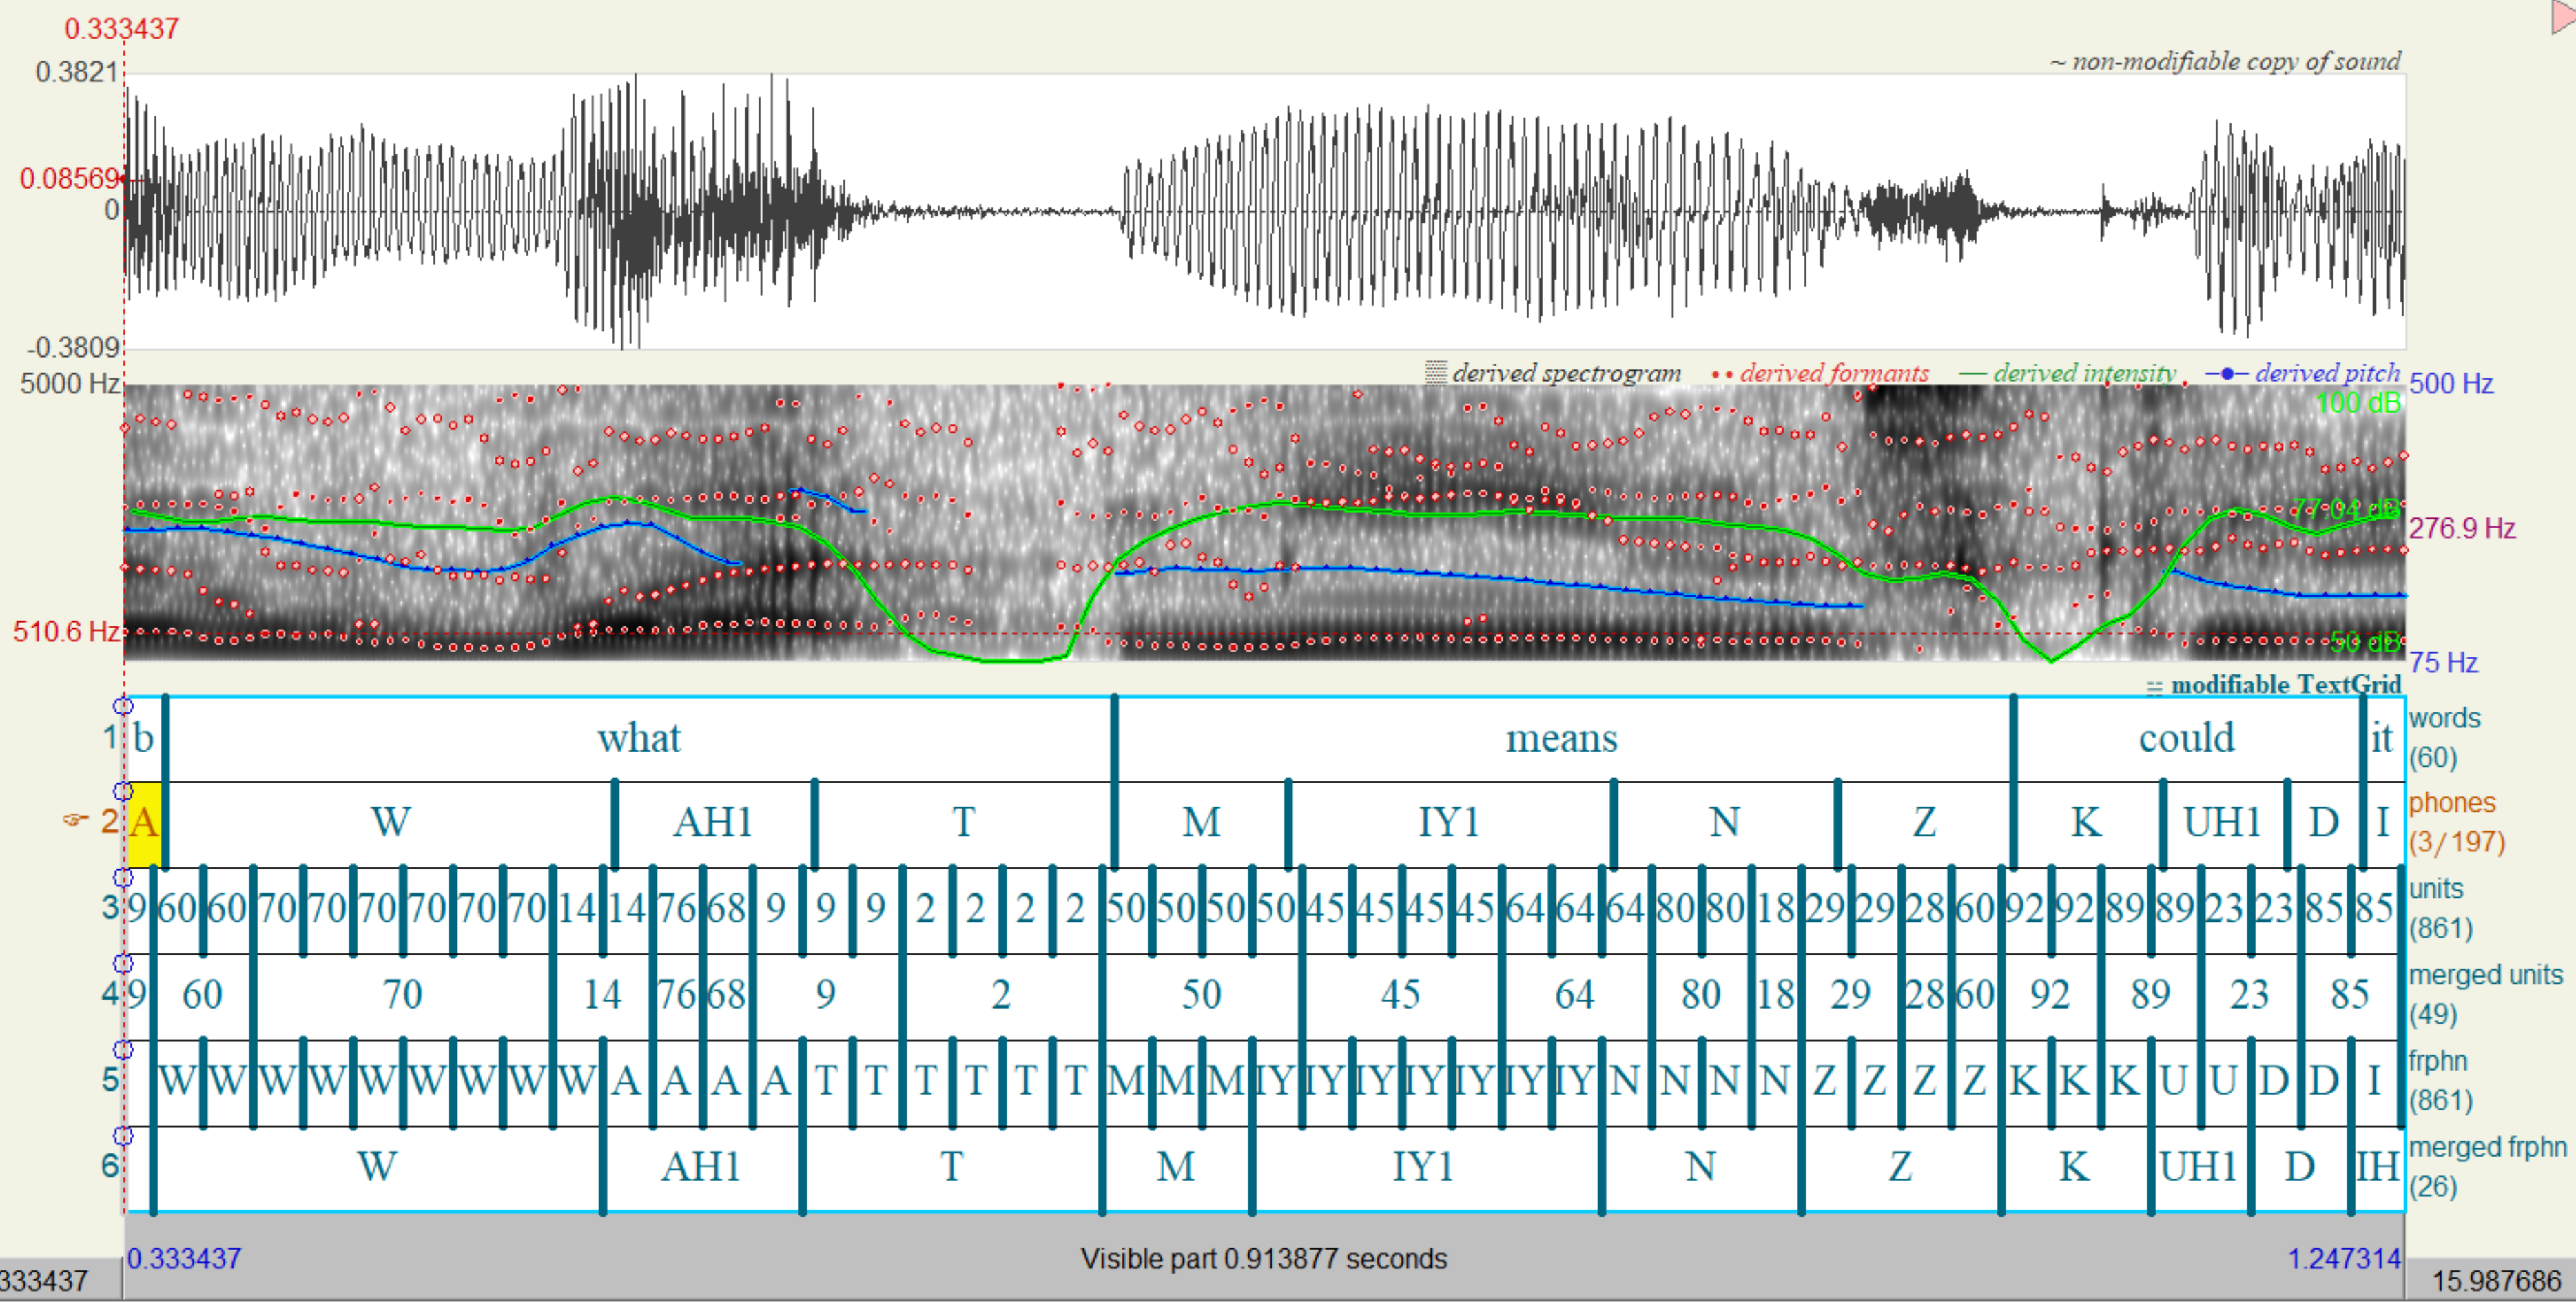
\includegraphics[width=1\linewidth]{figures/praat.png}
            \caption{以音框對齊的離散單元與音素標註範例}
            \label{fig:enter-labelwav}
        \end{figure}
        %%%%%%%%%%%%%%%%%
        
        此時若將整個待分析資料集的語音訊號全部蒐集起來,一共有 $T'$ 個音框,如此可分別獲得一個離散單元序列 $\boldsymbol{z} = \{z_t\}_{t=1}^{T'}$ 與音素標註序列 $\boldsymbol{y} = \{y_t\}_{t=1}^{T'}$ 進行統計分析。我們可以根據離散單元與標註之間配對的出現次數,寫為一個雙變數的共同分佈(Joint Distribution)
\begin{align}
    p_{yz} = \frac{\sum^{T'}_{t=1}[{y_t = i \wedge z_t = j}]}{T'}
\end{align}

其中 $i$ 是第 $i$ 個音位類別,而 $j$ 指編號為 $j$ 的離散單元。兩個變數的邊際機率(Marginal Probability)分別為
\begin{align}
    p_z(j) & =\sum_i{p_{yz}(i, j)} \\
    p_y(i) & =\sum_j{p_{yz}(i, j)}
\end{align}
因此,對於每一個音位 $i$ 而言,這個音位最可能的對應離散單元為
\begin{align}
    z^\ast(i) = \arg\max_j p_{yz}(i, j)
\end{align}
與之相對應的,對於每一個離散單元的類別 $j$ 則可以找到機率最高的音位
\begin{align}
    y^\ast(j) = \arg\max_i p_{yz}(i,j)
\end{align}
透過這些定義,以下分節介紹將要用來分析的指標。

\subsection{純度}

  本指標考慮音位和離散單元兩個序列之間對應的最高機率,因此從音位與離散單元的角度出發,可以得到以下兩項數據:

\paragraph{音位純度(Phoneme Purity)}\hfill \break
%
  考慮每個離散單元對應的音位中,最高機率音位的機率,表示為
\begin{align}
    \mathbb{E}_{p_z(j)}\left[p_{y|z}(y^*(j)|j) \right]
\end{align}
此指標表示該單元是否對其對應的音位有足夠的代表性。

\paragraph{分群純度(Cluster Purity)}\hfill \break
%
  與音位純度相對,改以每個音位的角度,考慮對應單元類別的機率
\begin{align}
    \mathbb{E}_{p_y(i)}\left[p_{z|y}(z^*(i)|i) \right]
\end{align}
        由於離散表徵進行分群演算法時的類別數是一項超參數(Hyperparameter),且通常離散單元的分群數量會比音位多,因此該統計數據本身不直接具有語音學的解釋意義,而且在分群數量很多時其數值會顯著下降。然而該指標在考量音位純度時必須一併考慮,因為當分群數非常多時,分群純度過低暗示離散單元做不到歸納音位類別的效果,使得音位純度失去其意義。一個極端的情形是每一個音框都給予不同的離散單元編號,如此音位純度可以達到100\%。

\subsection{熵和相互資訊}

  除了純度提供「最高機率」的對應關係,根據 HuBERT 論文 \cite{hsu_hubert_2021-2} 中的分析方式,我們也可以從資訊理論的角度,觀察兩個序列的熵和相互資訊。

\paragraph{熵(Entropy)} \hfill \break
%
  熵的定義按照資訊理論,衡量兩個序列中標籤類別出現機率的不確定性(Uncertainty),公式寫作:
\begin{align}
    H(y) & = \sum_i{p_y(i)\log p_y(i)} \\
    H(z) & = \sum_j{p_z(j)\log p_z(j)}
\end{align}
其中 $H(y)$ 和 $H(z)$ 分別為音位和離散單元的熵,數值愈高分別表示各種音位和離散單元出現的機率愈平均。

\paragraph{以音位標準化之相互資訊(Phone-normalized Mutual Information,PNMI)}\hfill \break
%
  本數據以「觀察到某一個離散單元,能降低多少音位標註的不確定性」,定義該離散單元的出現背後提供了多少音位的資訊。公式寫為:
\begin{align}
    \frac{I(y;z)}{H(y)} & =\cfrac{\sum_i \sum_j p_{yz}(i, j) \log \cfrac{p_{yz}(i, j)}{p_y(i)p_z(j)}}{\sum_i p_y(i) \log p_y(i)} \\
                        & =\frac{H(y)-H(y|z)}{H(y)}                                                                              \\
                        & =1-\frac{H(y|z)}{H(y)}
\end{align}
        該項數據愈高,表示離散單元的分群愈能提供語音音位的資訊,是一個品質更好的分群結果。由於離散單元是否能夠正確對應到音位才是人們所關心的問題,因此與純度不同,只以音位的角度出發,而不考慮以離散單元分群的角度。

\section{語音學的音位分類(Phoneme Type)}

  除了單一音位本身的特性以外,由於音位之間存在相似的特徵,可以分成幾個組別。這裡依照希氏(Sicherman) \cite{10097097}、阿氏(Abdullah)\cite{abdullah23_interspeech} 等前作的分組方式,對英語的音位進行分類。如此一來,除了單純把音位標註以約 40 類完全獨立的標籤看待,還能夠觀察這些離散單元是否有擷取到相似的發聲特徵。首先,按照發音過程氣流是否受到阻礙,因此可否形成獨立的音節,音位可以分為輔音與元音兩大類,而後再根據發音的細部特性共分成七組。

\paragraph{輔音(Consonant)} \hfill \break
  
        輔音是指透過阻擋氣流發聲的音位,因此通常不單獨構成音節,
按照發音方式可分為以下五個類別:
        
        \begin{itemize}
            \item 塞音(Plosive):以完全阻塞氣流的方式發音的音位,包含 /p/、/b/、/t/、/d/、/k/、/g/ 六種。
            \item 擦音(Fricative):藉由在口腔中形成的縫隙,使氣流通過時摩擦形成的發音,包含 /f/、/v/、/s/、/z/、/\textesh/ (sh)、/\textyogh/ (如「garage」的 「-ge」)、/θ/ (無聲的 th)、/ð/ (有聲的 th)、/h/ 九種。
            \item 塞擦音(Affricate):由塞音和同部位的擦音同時發出的輔音,英語中只有 /t\textesh/ 和 /d\textyogh/ 兩種,即 ch 和 j 的發音。
            \item 鼻音(Nasal):使氣流通過鼻腔形成的聲音,有 /m/、/n/、/ŋ/ (ng) 三種。
            \item 近音(Approximant):又稱半元音,為介於元音和輔音之間的聲音,有 /j/ (為 y 作為輔音時的發音)、/r/、/l/、/w/ 四種。
        \end{itemize}

\paragraph{元音(Vowel)} \hfill \break
  
        與之相對,元音則是不阻礙氣流通過,因此可自成音節的音位。其中又可分為發音位置固定的單元音(Monophthong)和會移動發音位置的的雙元音(Diphthong)兩類。通常以 a、e、i、o、u 字母產生的聲音皆屬於此類別。
        
        透過將音位分成以上七組後,並重新分析統計指標,以觀察這些分組的規律如何在離散單元的出現機率上呈現,進而顯示離散單元是否與語音的發音方式具有一定的關聯性。

        另外,為了方便統計與作圖,這些音位在圖中並非以語言學慣用之國際音標(International Phonetic Alphabet,IPA)\cite{international1999handbook},而是參考語音處理領域常用的「卡內基梅隆大學發音辭典(Carnegie Mellon University Pronouncing Dictionary,CMUDict)\cite{noauthor_cmu_nodate}」,取用其中的 ARPABet 表示法 \cite{klautau2001arpabet},以避免字母以外的符號在處理上的困難。表 \ref{tab:ipa1}、\ref{tab:ipa2} 中列有更詳細的音位資訊\footnote{範例單詞取自 CMUDict 官網說明。}。


\newcommand{\myipatablename}[0]{英語音位的 ARPABet 表示法和音位分類資訊}

\begin{table}
    \centering
    \begin{tabular}{|c|c|c|c|c|} \hline
        音位 & ARPABet 表示法 & 音位分類 & 範例單詞 & 範例單詞的音位\\ \hline\hline
/\textipa{A}/ & AA & 單元音 & odd  &   AA D \\ \hline
/\textipa{\ae}/ & AE & 單元音 & at & AE T \\ \hline
/\textipa{2}/ & AH & 單元音 & hut &     HH AH T \\ \hline
/\textipa{O}/ & AO & 單元音 & ought &   AO T \\ \hline
/a\textipa{U}/ & AW & 雙元音 & cow &     K AW \\ \hline
/a\textipa{I}/ & AY & 雙元音 & hide &    HH AY D \\ \hline
/b/  & B  & 塞音 & be & B IY \\ \hline
/t\textesh/ & CH & 塞擦音 & cheese &  CH IY Z \\ \hline
/d/  & D  & 塞音 & dee &     D IY \\ \hline
/\textipa{\dh}/ & DH & 擦音 & thee &    DH IY \\ \hline
/\textipa{E}/ & EH & 單元音 & Ed & EH D \\ \hline
/\textrhookrevepsilon/ & ER & 單元音 & hurt &    HH ER T \\ \hline
/\textipa{E}\textipa{I}/ & EY & 雙元音 & ate &     EY T \\ \hline
/f/  & F  & 擦音 & fee &     F IY \\ \hline
/\textscriptg/  & G  & 塞音 & green &   G R IY N \\ \hline
/h/ & HH & 擦音 & he & HH IY \\ \hline
/\textipa{I}/ & IH & 單元音 & it & IH T \\ \hline
/i/ & IY & 單元音 & eat &     IY T \\ \hline
/d\textyogh/ & JH & 塞擦音 & gee &     JH IY \\ \hline
/k/  & K  & 塞音 & key &     K IY \\ \hline
    \end{tabular}
    \caption{\myipatablename }
    \label{tab:ipa1}
\end{table}

\begin{table}
    \centering
    \begin{tabular}{|c|c|c|c|c|} \hline
        音位 & ARPABet 表示法 & 音位分類 & 範例單詞 & 範例單詞的音位\\ \hline\hline
/l/  & L  & 近音 & lee &     L IY \\ \hline
/m/  & M  & 鼻音 & me & M IY \\ \hline
/n/  & N  & 鼻音 & knee &    N IY \\ \hline
/\textipa{N}/ & NG & 鼻音 & ping &    P IH NG \\ \hline
/\textschwa\textipa{U}/ & OW & 雙元音 & oat &     OW T \\ \hline
/\textipa{O}\textipa{I}/ & OY & 雙元音 & toy &     T OY \\ \hline
/p/  & P  & 塞音 & pee &     P IY \\ \hline
/r/  & R  & 近音 & read &    R IY D \\ \hline
/s/  & S  & 擦音 & sea &     S IY \\ \hline
/\textesh/ & SH & 擦音 & she &     SH IY \\ \hline
/t/  & T  & 塞音 & tea &     T IY \\ \hline
/\texttheta/ & TH & 擦音 & theta &   TH EY T AH \\ \hline
/\textipa{U}/ & UH & 單元音 & hood &    HH UH D \\ \hline
/u/ & UW & 單元音 & two &     T UW \\ \hline
/v/  & V  & 擦音 & vee &     V IY \\ \hline
/w/  & W  & 近音 & we & W IY \\ \hline
/j/  & Y  & 近音 & yield &   Y IY L D \\ \hline
/z/  & Z  & 擦音 & zee &     Z IY \\ \hline
/\textyogh/ & ZH & 擦音 & seizure & S IY ZH ER \\ \hline

    \end{tabular}
    \caption{\myipatablename(續)}
    \label{tab:ipa2}
\end{table}


\section{實驗集與分析模型}

  本研究的分析對象參考無文字架構 \cite{noauthor_textless_2021, lakhotia_generative_2021, lakhotia_generative_2021-1} 的研究,
採用論文中提及的四種語音表徵,簡述如下:

\begin{itemize}
    \item CPC \cite{rivière2020unsupervised}:卷積式編碼器 + 遞迴式預測器,以對比式學習訓練。表徵來自預測器的中間層,每 10 毫秒提取一個向量表徵作為音框
    \item Wav2vec 2.0 \cite{baevski2020wav2vec}:卷積式編碼器 + 轉換器預測器,以對比式學習訓練。表徵來自轉換器第 14 層,每 20 毫秒作為一個音框
    \item HuBERT \cite{hsu_hubert_2021-2}:卷積式編碼器 + 轉換器預測器,以預測式學習訓練,其訓練目標為 K-平均分群演算法的結果,透過遮蔽語言模型的方式訓練。表徵來自轉換器第 6 層,每 20 毫秒作為一個音框
    \item LogMel:為 80 維對數梅爾時頻譜的聲學特徵,在此作為比較基線(Baseline)。音框寬度為 10 毫秒
\end{itemize}

        我們跟隨拉氏等人所提出的無文字架構 \cite{lakhotia_generative_2021-1} ,使用該篇論文中釋出之預訓練模型與 K-平均量化模型,預訓練模型的設定細節於原論文有更詳細的描述,而量化模型則是拉氏等人透過公開的 LibriSpeech 資料集 \cite{panayotov_librispeech_2015} 中之 train-clean-100 訓練子集,獲取語音表徵後執行 K-平均分群演算法所得,並釋出群數為 50、100 和 200 的三個版本。

        本論文以 LibriSpeech 之 train-clean-100 訓練子集作為分析對象,將語音語料庫的語音資料經過四個模型得到連續表徵後,再經過量化模型得到完全由離散單元組成的「虛擬文字」語料。至於音位標註的取得,則是透過強迫對齊器\footnote{https://github.com/MontrealCorpusTools/Montreal-Forced-Aligner}的英語預訓練模型,將語料庫的文字轉寫轉換為帶有對應時間範圍的音位標註資料,並依據各自語音表徵的時間解析度,生成以音框對齊的音位標註語料,隨後進行相關性的分析。

}

\section{分析方式}

  針對模型得出之離散單元與音位標註之間的對應關係,為了更直觀的解釋這些指標的意義,並且看清楚這些數字背後之間代表的現象與細部特徵,我們將音位與離散單元的共同機率分佈 \(p_{yz}\) 用熱圖(Heatmap)呈現,來解釋這些指標的意義,並以此進一步往下深入探討。

        首先,這裡以 HuBERT 為基石模型、離散單元分群數為 50 的統計數據為例,圖 \ref{fig:hubert-50-joint-byprob} 說明我們如何分析語音離散表徵與音位標註的關係。

\begin{figure}
    \centering
    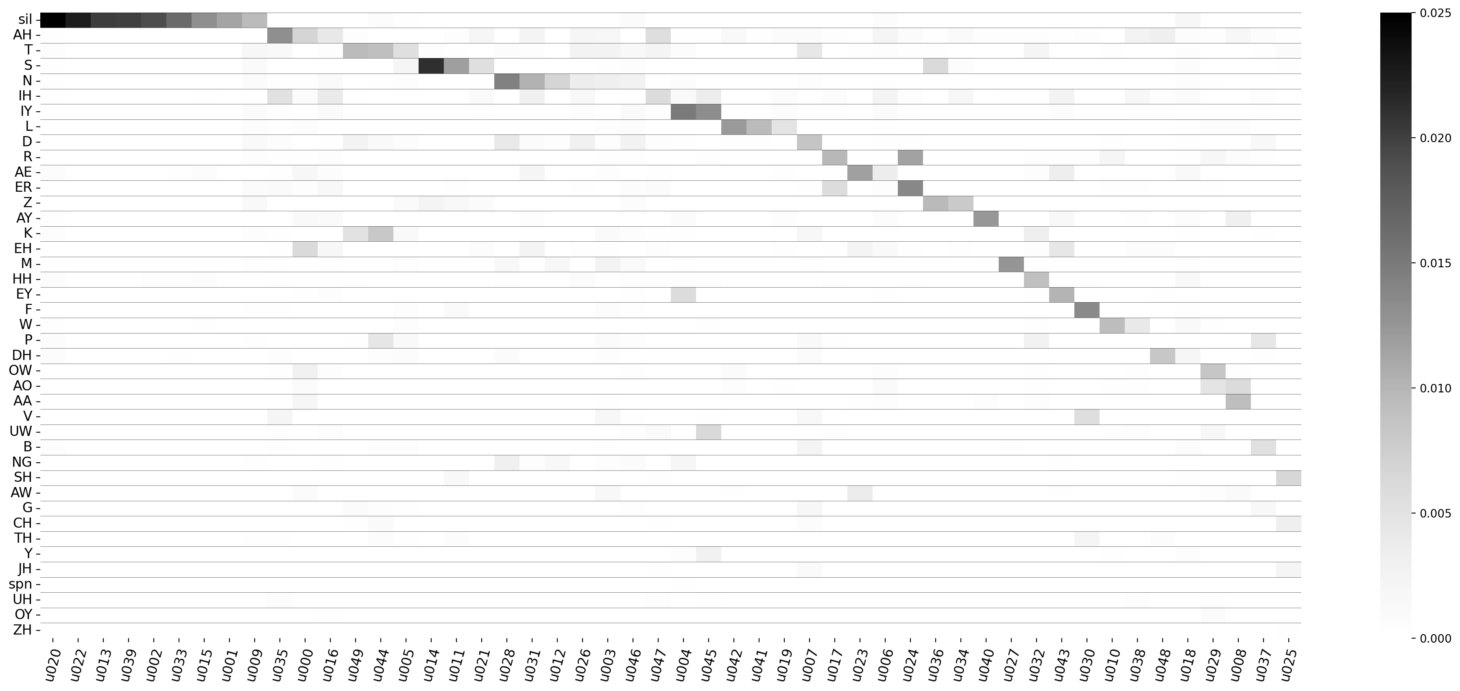
\includegraphics[width=1\linewidth]{figures/hubert-50-joint-byprob.png}
    \caption{HuBERT 模型、分群數為 50 之 \\
    離散單元與音位標註的共同機率分佈圖}
    \label{fig:hubert-50-joint-byprob}
\end{figure}

        圖中的縱軸表示各個音位,橫軸表示各個離散單元。在這張圖中,縱軸的音位是按照其邊際機率 \(p_y(i)\) 由高至低排序;橫軸的離散單元則是依據其對應的最高機率音位 \(y^\ast(j)\) 的縱軸排序位置進行排列。\footnote{如果兩個離散單元 \(j_1\) 和 \(j_2\) 對應到相同的音位 \(y^\ast = y^\ast(j_1) = y^\ast(j_2)\),則依照機率值 \(p_{yz}(y^\ast, j_1)\) 和 \(p_{yz}(y^\ast, j_2)\) 由高到低進行排序,對於多個離散單元的情況以此類推。} 這樣可以在熱圖上呈現出由左上至右下的對應關係。

        為了評估離散表徵是否有捕捉到與音位相關的資訊,我們可以分別從音位與離散單元的兩個角度出發,考慮以下兩個問題:
\begin{enumerate}
    \item 對於每個音位而言,它們所對應的離散單元集中程度如何?
從這個角度出發,可以觀察不同音位的集中程度,進而推論模型是否能夠辨認出該音位的發音特性,藉由給予夠高的一致性將這些語音訊號分類在一起。會不會有某一些音位很難被歸類出來?
    \item 反之,一個離散單元所對應的音位的集中或分散程度如何?
如果一個音框的語音訊號被模型指示為特定的離散單元,該單元作為虛擬標註,能多大程度的對應到人耳感知的音位標註?也就是這些虛擬標註,是否達成音位標註類似的效果,足以把不同語音特徵區分開來。
\end{enumerate}

        這兩個問題的答案可以分別很直觀的從圖中顏色的深淺觀察出來,也正好對應前面所提及的兩個純度指標:
        \begin{enumerate}
            \item 將每個橫列(Row)取最大值相加後的總和即為分群純度
            \item 將每個直行(Column)取最大值相加後的總和則是音位純度
        \end{enumerate}

        從這裡我們可以看到,當分群數量增加時,音位純度可以在每個直行上取到更多的機率值,這也意味著當分群數量與音框數量相同時,音位純度可以達到 100\%,與前面的描述互相吻合。另一方面,當分群數量增加時,每個格子的機率值會因為離散單位數量的增多而被稀釋,而分群純度受到音位數量限制,只能取 41 個 $p_{yz}$ 值的總和,使得單位純度因而明顯降低。

        以上是綜觀整個系統給予虛擬標註時,對應到音位標註的好壞。然而我們可以更進一步的探討各音位與離散單元之間的內部差異,也就是分別探討:
\begin{itemize}
    \item 哪些離散單元比較能集中抓取音位的特徵,不會與其他音位混淆?
    \item 如果一個離散單元被分散的對應到多個音位,那麼這些音位可能是哪幾個?是否存在某些共同特徵?
\end{itemize}

        由於這些問題是以離散單元的角度出發,因此我們仿照前作如 SpeechTokenizer \cite{zhang2024speechtokenizer}、DinoSR \cite{liu2024dinosr} 的作法,將熱圖改以 $p_{y|z}(i|j)$ 呈現,即對每個直行進行標準化得到條件機率,以顯示每個單位對應到哪個音位,探討這種對應如何集中或分散。

\begin{figure}
    \centering
    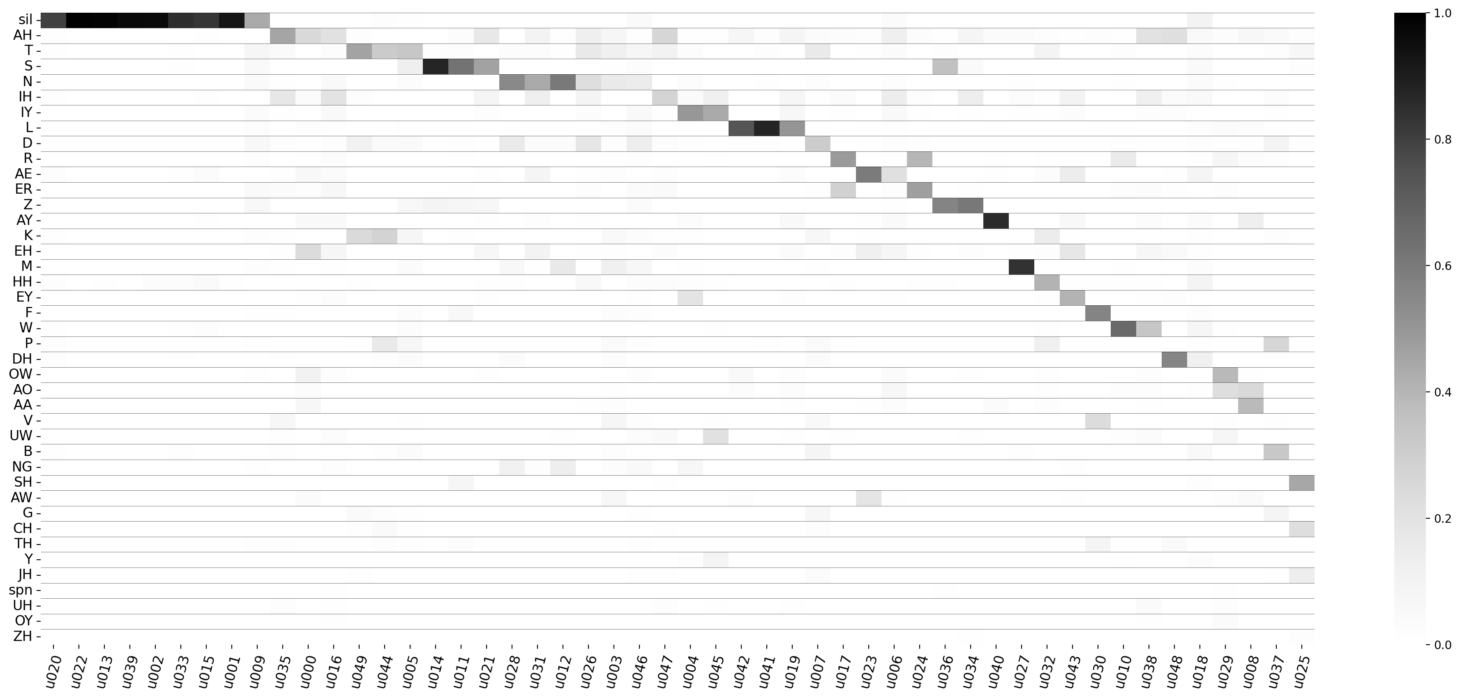
\includegraphics[width=1\linewidth]{figures/11111111.png}
    \caption{HuBERT 模型、分群數為 50 之\\
$p_{y|z}(i|j)$  條件機率分佈圖}
    \label{fig:hubert-50-givenunit-byprob}
\end{figure}
        從圖 \ref{fig:hubert-50-givenunit-byprob} 中可以更明顯的看出,模型會耗費不少種類的離散單元於編碼非音位的音素標註(尤其是 sil)之上。\jeffcomment{加上 silence ratio?}此外,每個離散單元對於其對應的訊號所對應的音位集中程度有高有低,使得音位純度無法到達 1.00。然而,這邊比較有趣的點是,觀察那些對應音位比較分散的離散單元,我們其實可以發現這些音位彼此之間有很強的關聯性,幾乎與前述的語音分類一致。  % 

        \begin{figure}
            \centering
            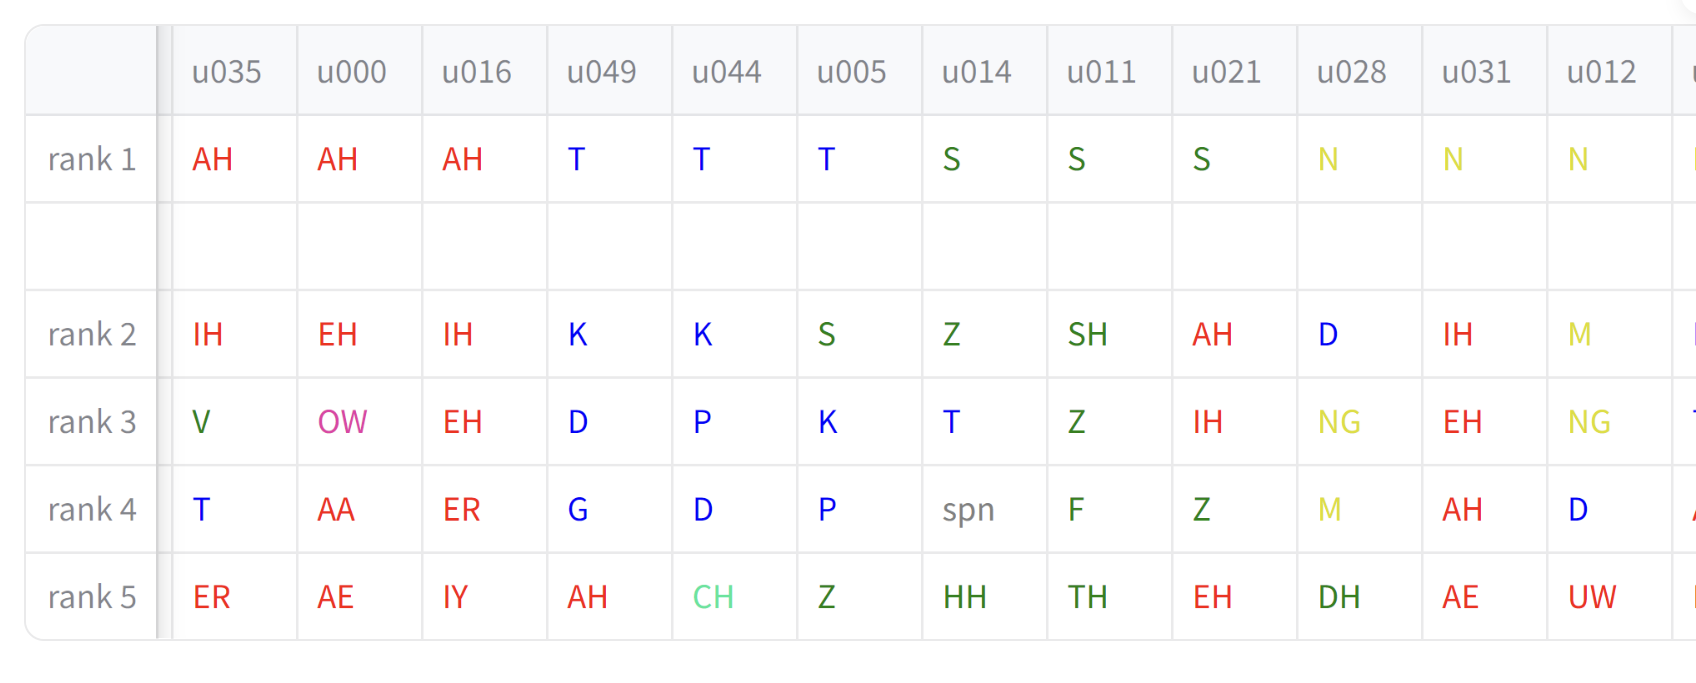
\includegraphics[width=1\linewidth]{figures/unit_rank_phn.png}  % figures/unit_perspective.png
            \caption[]{
離散單元對應的前幾高音位示意。圖中的方框、圓圈等形狀}
                                          表示輔音發聲部位,外框顏色則表示清濁音。注意元音都屬於濁音
            \label{fig:unit-to-phn-rankings}
        \end{figure}
        
        這件事可以從熱圖上由左上而右下連線中,不在線上但顏色較深的區塊中觀察出來。但由於直接從熱圖上觀察比較難以呈現,因此我們另外統計出表 \ref{fig:unit-to-phn-rankings},其中展現的是幾個離散單元對應的前五高機率音位,並且用顏色標明各音位所屬的語音學類別。從表中大致可以看出以上描述的趨勢,而且即便不是同一個語音學類別,按照前面講解語音學對音位歸類的另外兩個層面 --- 發音部位和清濁音,還是可以將各離散單元的前幾名之中盡量找出共通點。例如 05 號單元對應的前兩名 /t/ 和 /s/ 雖然並不屬於同一個發聲方式,因而被分成兩個類別,但如果從國際音標表中的「發音部位」來觀察,會發現它們都屬於「齒音」。換言之這些離散單元捕捉到的語音特性是多個面向的,並不僅限於單一的分類方式,而是可以對應到國際音標表上至少兩個維度以上的類型。

\begin{figure}
    \centering
    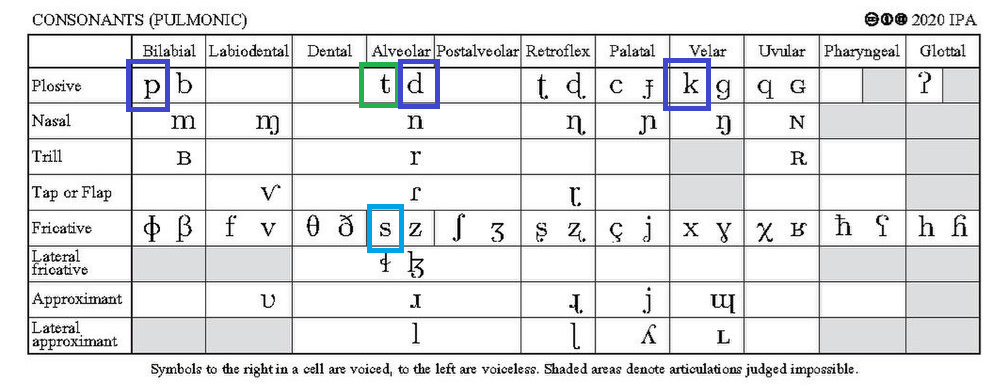
\includegraphics[width=1\linewidth]{figures/ipa_similarity.png}
    \caption[]{
國際音標表的輔音表格,說明離散單元}
                                                                對語音聲學特徵的捕捉並不僅限單一面向
    \label{fig:ipa-cons-table-sim}
\end{figure}

        透過以上的觀察,因此我們有足夠的理由重新對熱圖的縱軸重新排列,並按照語音學分類進行分組,來觀察這些離散單元是如何指示出音位之間的相似性,區分出同個音位、同類發音,或者如何被混淆為其他類別,而這些類別是否有某些特徵,最後這樣的現象是否只在單一模型出現,抑或是在不同的離散單元系統都會發生。

\begin{figure}
    \centering
    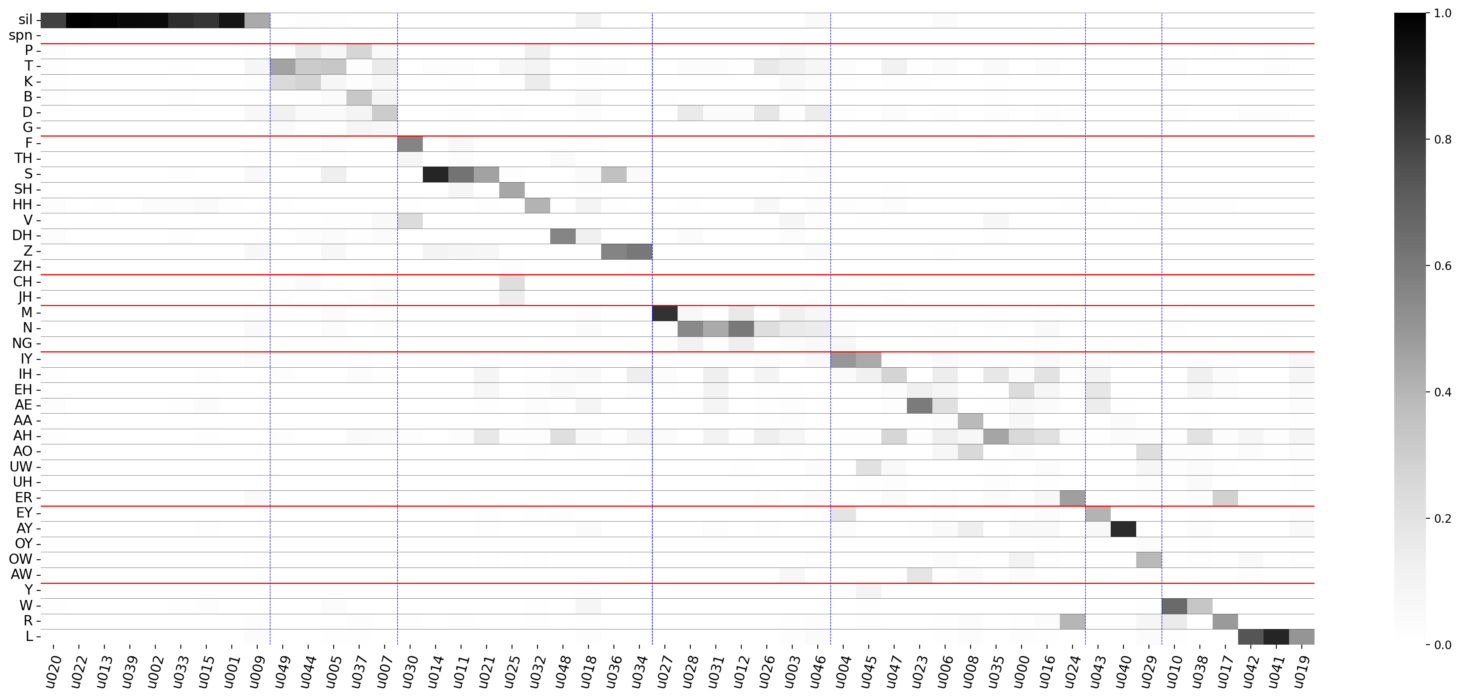
\includegraphics[width=1\linewidth]{figures/hubert-50-givenunit-byphn.png}
    \caption[]{% \medskip % \small
        HuBERT 模型、分群數為 50 之離散單元}
                                                    與音位標註的條件機率,依照語音學分類排序的分佈圖
    \label{fig:hubert-50-givenunit-byphn}
\end{figure}

        這張圖的分組順序是依照韋氏(Wells) \cite{wells_phonetic_2022} 論文中的出現順序排列,而組別內則是清音在上、濁音在下,而同樣清濁音則是以發音位置由前往後排列。除了縱軸上按照音位本身特性分組,依循純度中使用的「代表音位」 $i^\ast$ 概念,我們同樣也對每個離散單元的代表音位排序,並且也依照這些代表音位進行分組觀察。

        為了比較好的刻劃這個在分群內的好壞,我們接下來多算兩個指標:\par
\begin{enumerate}
    \item 語音分類的純度:為了確認每個離散單元如何「將音位至少分到同一語音學類別」的程度,藉由將前面音位純度的式子,但將音位標註改為語音學類別,便可以求得這個數據。
    \item 各發音類別的純度:為了衡量模型對於每個類別內部區分不同音位的能力,比較模型對於不同組別區分音位的難易度,我們可以根據音位的語音學類別,將所有的音框等效分成八份語料後,分別再次統計純度(亦即計算對語音學類別取條件機率後計算純度)。
\end{enumerate}

        說明完以上指標後,我們將展示不同離散表徵模型的所有分析,彼此先進行綜觀比較,此後再針對細部的特徵分析。


}
\section{分析結果}

\subsection{不同語音離散表徵的比較}

  首先是比較不同模型的離散特徵之數據與機率分佈圖:

純度:
{

\begin{figure}
    \centering
    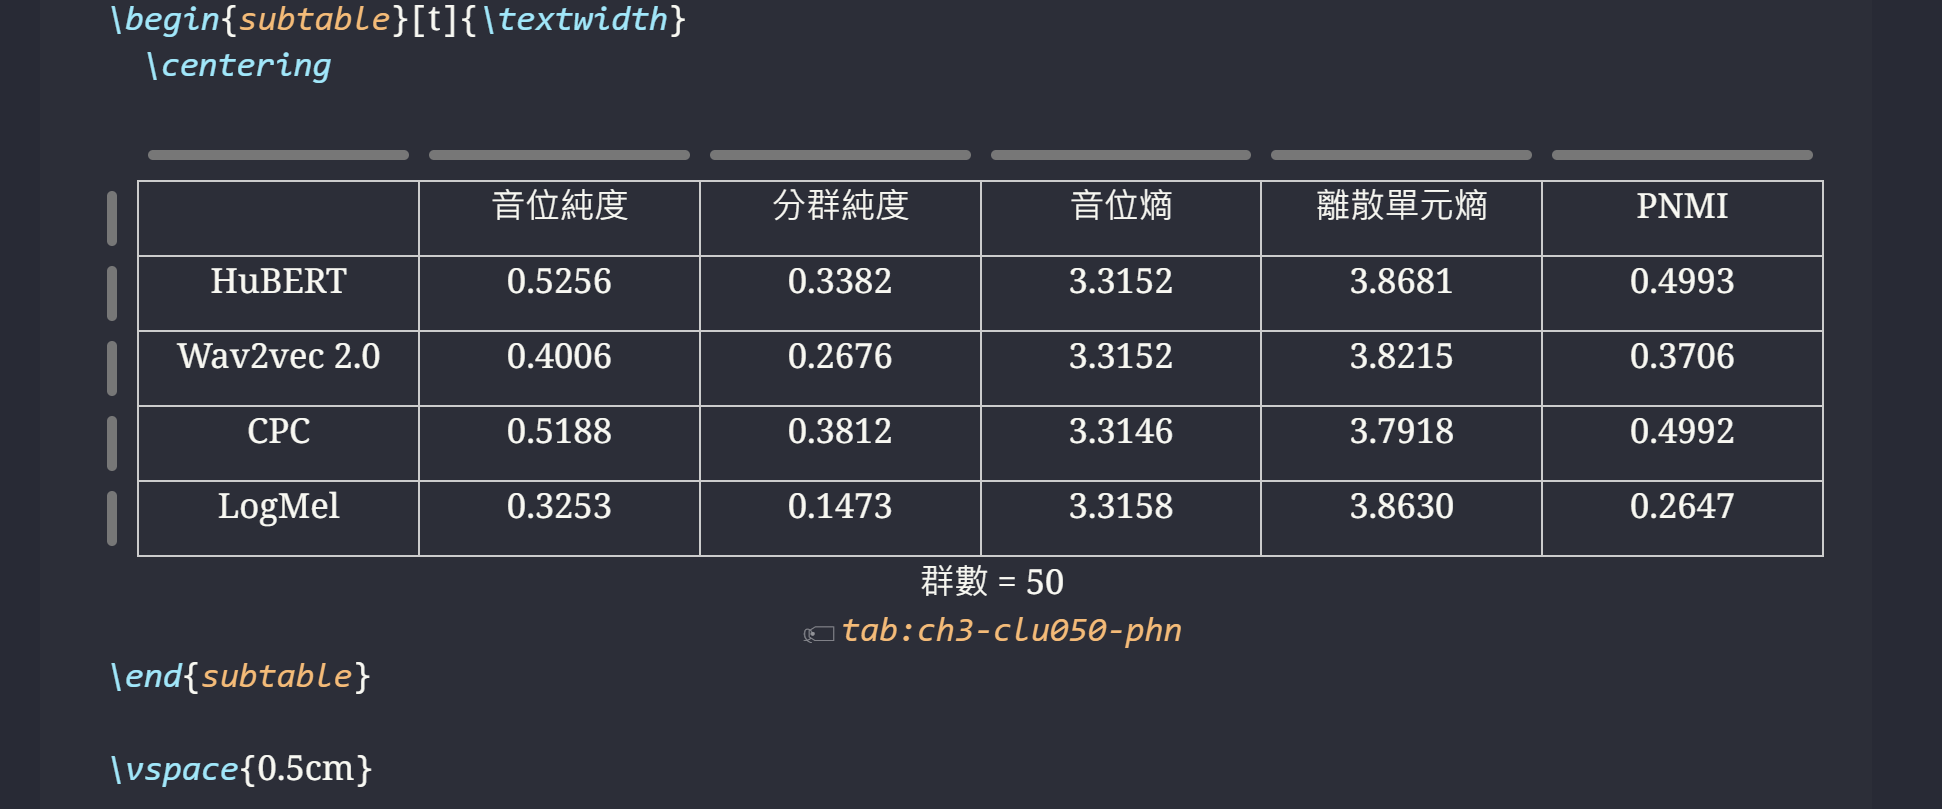
\includegraphics[width=1\linewidth]{figures/000.png}
    \caption{比較表}
    \label{fig:enter-label}
\end{figure}

}
機率分佈圖:
{

\begin{figure}
    \centering
    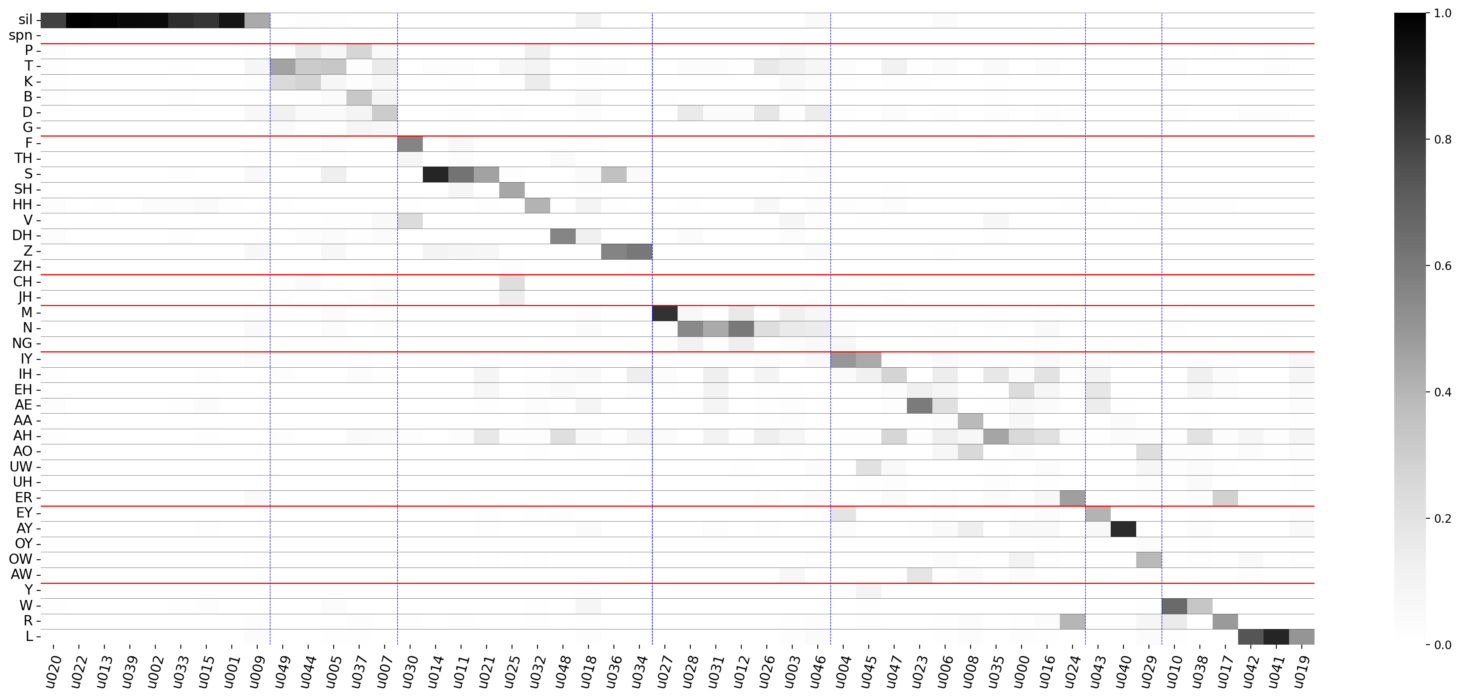
\includegraphics[width=1\linewidth]{figures/hubert50.png}
    \caption{Hubert}
    \label{fig:enter-label}
\end{figure}
\begin{figure}
    \centering
    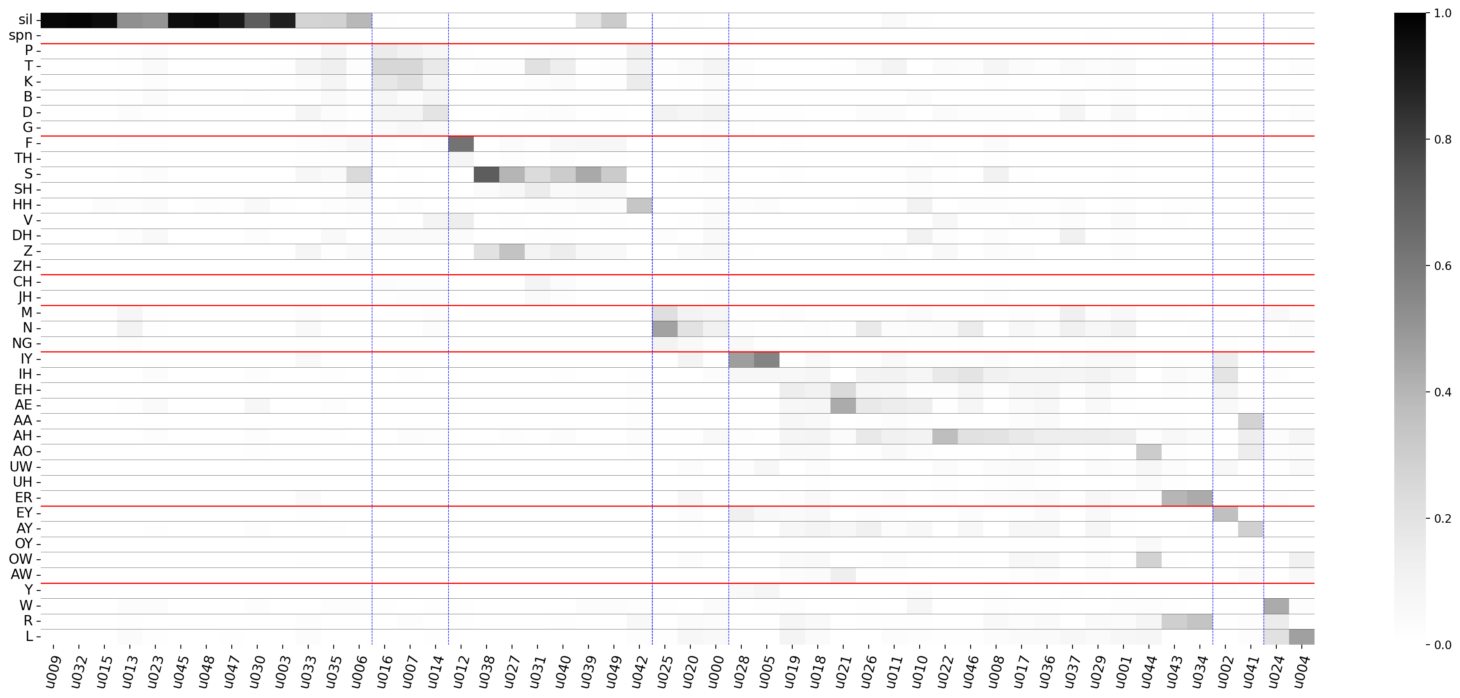
\includegraphics[width=1\linewidth]{figures/w2v250.png}
    \caption{w2v2}
    \label{fig:enter-label}
\end{figure}

\begin{figure}
    \centering
    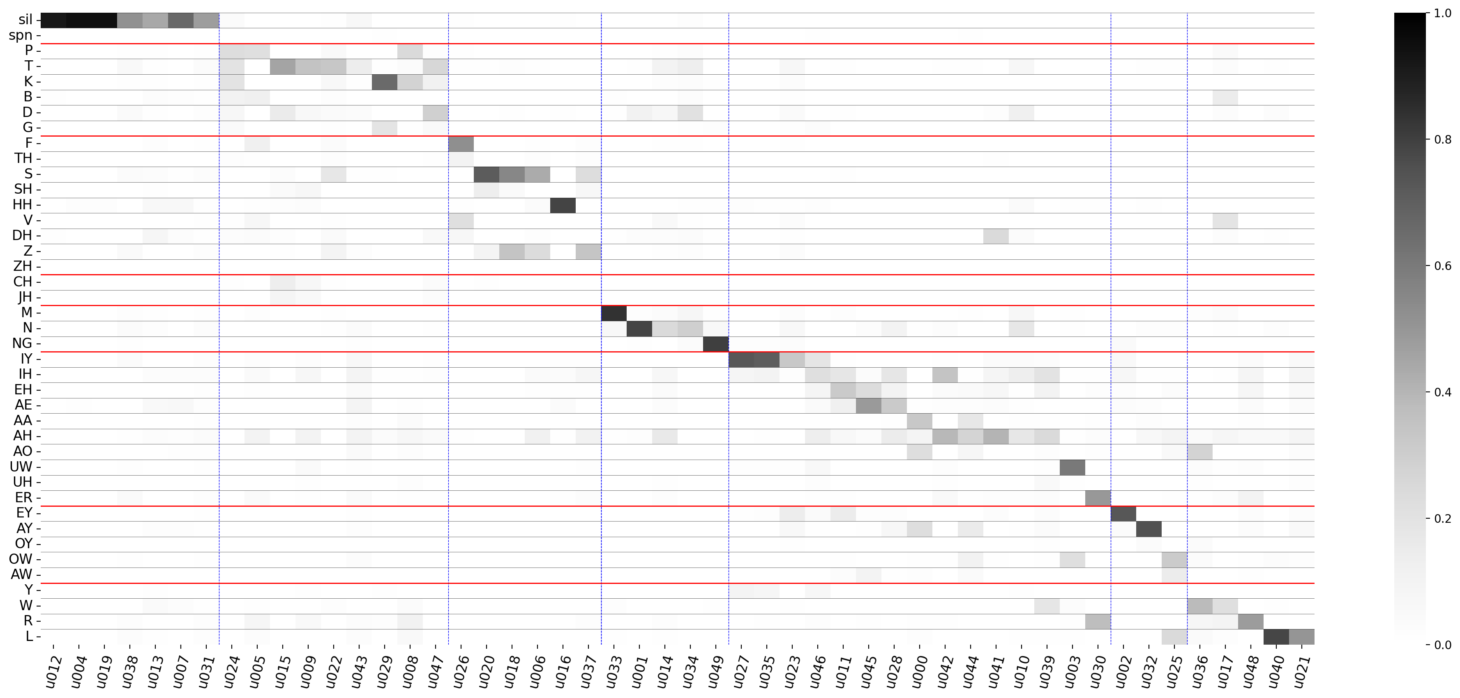
\includegraphics[width=1\linewidth]{figures/cpc50.png}
    \caption{cpc}
    \label{fig:enter-label}
\end{figure}

\begin{figure}
    \centering
    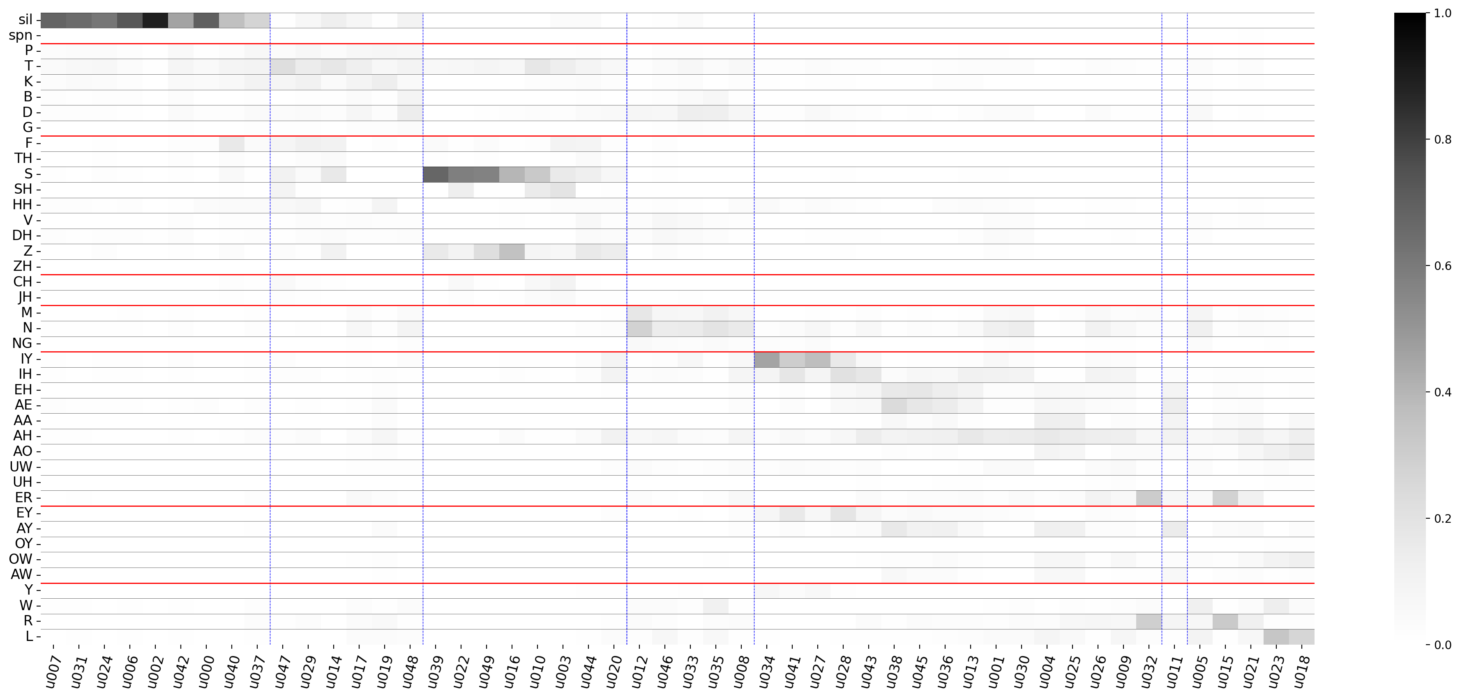
\includegraphics[width=1\linewidth]{figures/logmel50.png}
    \caption{logmel}
    \label{fig:enter-label}
\end{figure}

}

        比較不同的模型的聯合分佈後,我們可以觀察到這些模型之間,確實存在。

        就是說標注跟單元之間的 相關性 高低,比較,從聯合分佈圖上也可以明顯的呈現出來,進而說明這些不同的語音離散表徵之前,捕捉訊號中的發音特徵能力的強弱。從圖中可以看出,HuBERT 跟 CPC 的效果比另外兩種表徵好上不少。

        此外,我們也可以比較同一種語音表徵之下,不同的離散單元分群數之間對於音位特徵捕捉的強弱程度。基於前面表徵純度與相互資訊的考量,這邊固定用 HuBERT 當比較對象。從這三種分群數看來,離散單元數量愈多,愈能夠區分出比較細節的語音類別。例如,如果要從每個 離散單元 的代表音位來觀察,要至少有 100 個群數,才至少有一個離散單元能代表塞擦音。如果分群數量太少,很多細節的發音音位則很容易被放在一起,難以區別出更細節的發音差異。

        再者,我們觀察到模型會消耗一定比例的離散單元去代表非音位的發音,以此我們計算出一個「非音位比例」,也就是等效有幾個 離散單元 被拿去代表這些不是音位的聲音。具體算法是使用 $E [ u | p ] $  總和除以離散單元的數量。

        然後,我們期望看到一個單元系統怎麼有效的去使用這些離散單元,因此我們可以畫一張離散單元音位熵的直方圖(Histogram)來刻劃模型系統在使用這些離散單元的集中程度。如果整體向熵值低處偏,表示模型的各種離散單元所代表的音位都是相對確定的,也就是更好的捕捉到了音位特徵。

        最後,為了觀察各自不同語音學類別內分群的好壞,我們可以算語音學類別的純度,並且再以各個語音學類別區分出來,計算八個類別的各自 條件機率下計算的 純度,以此比較不同表徵、分群數在針對不同語音學類別的特徵補綴效果。

        比較完這些表徵與離散單元數量的各項綜觀統計指標後,我們基於 相互資訊 和 純度 的高低,著重關注於 HuBERT 100 和 50 模型或 CPC,藉由觀察和比較兩個模型共有的規律,往下細部探討該模型所捕捉到的離散單元和音位之間的關係。

\subsection{個案探討}  % 分組討論  %

  首先,承接前面所述的「熱圖上不在斜線上的點」,我們可以觀察每個離散單元所對應的 音位 之間的共同特性。

        接著,我們確認一下對應最紛亂與最集中的幾個 離散單元 的狀況。

        接著,跟隨韋氏(Wells)\cite{wells_phonetic_2022} 之前的作法,我們觀察各類別的 音位 可能各自是以那些離散單元為代表。

        之後,從各個 音位 的熵值來觀察,我們可以發現\textcolor{red}{某某某某某}幾個音位的熵值特高特低,來發現這些音位可能是比較難以捕捉的。而這個現象在 50 模型又可能是怎樣怎樣的。

\subsubsection{切塊出來}

  最後,基於我們已經有對語音學分類,我們可以觀察熱圖上不同語音學類別所切出來的區域的亂度,來觀察各類別的發音特徵捕捉的難易度。例如塞音怎樣怎樣啊……

{


\section{本章總結}

  本章節探討以音框為單位取出的語音離散表徵與對應的音位標註之間的關係,從分析結果中可以看到,HuBERT 模型的離散表徵確實與人類理解的語音單位「音位」之間具有最明顯的相似性,也進一步證明為何 HuBERT 是抽取語音離散表徵時最常使用的模型。

        然而,單一離散表徵僅能代表 10 或 20 毫秒的語音訊號,而音位的長度經常佔據不只一個離散表徵。因此,下一章節將進一步組合多個離散表徵成為符記,分析它們與音位之間的關係。

%   從統計數據出發,我們針對聯合分佈的各個面向,配合了語音學知識的分類進行了細部探討,發現了 hunert 模型怎樣怎樣,而這件事可能在其他的模型之中差不多是 holid 住的。然後,因為 hunert 本身捕捉的各項純度與 MI 明顯較高,以此可以驗證為什麼 HuBERT 的離散單元可以在無文字架構內被當成類似音位或文字的表徵,並進而套用於語音語言模型的訓練上,同時為許多做語音模型解釋性的作品所關注citehao。


}
